%-----------------------------------------------------------------------------------------------
\chapter{Quad detection}\label{sect:quad_detection}
%-----------------------------------------------------------------------------------------------

In this chapter there will be a summary of the image processing algorithms tried and used for the recognition of the fiducial markers.
From a computer vision point of view the task is to detect joint line segments.
This is a well researched task in image processing, there are many well tried algorithms for it.

In this chapter will be a short summary of the algorithms used for testing and performance comparison.


The general flow of processing is the same for every line fitting solution.


The process here diverges depending on which line fitting algorithm is used.
They all need differently conditioned input images for optimal performance.
The line fitter routines not necessarily have the same output format\footnote{Some return line segments defined by their endpoint, others use the polar representation of a line etc.}, so conversion may be needed.
This is the end of the marker recognition phase.
This step of the process takes the raw input image and initiates quad structures based on the observed picture.

Three separate line fitting techniques and their variants were profiled in this experiment.
\begin{itemize}
	\item Hough-transformation
	\item Corner detection
	\item Line Segment Detector\cite{LSDDet}
\end{itemize}
The first one uses the Hough-transformation for line detection.
There are many variants of the transformation: Standard Hough Transform, Probabilistic Hough Transform, Multiscale Hough Transform, etc...
The 2 most commonly used are the standard- and the probabilistic variants.
The OpenCV framework offers implementations for them, both were tested in the experiment.

The second detector is based on corner recognition.
There are more variants of this method to try out, too.
The corner metrics of a feature can be calculated differently with (Harris metric, eigenvalues, etc.) varying results.
It is also needed for the solution to be scale invariant, which also can be achieved in a number of ways.

The third alternative is the Line Segment Detector algorithm described in \cite{LSDDet}.
It is a robust and fast algorithm for detecting line segments on an image.
The OpenCV framework provides an implementation of it as well.

A typical marker shot with partial visibility is shown figure \figref{partialMarkerShot}.
\begin{figure}[ht]
	\centering
	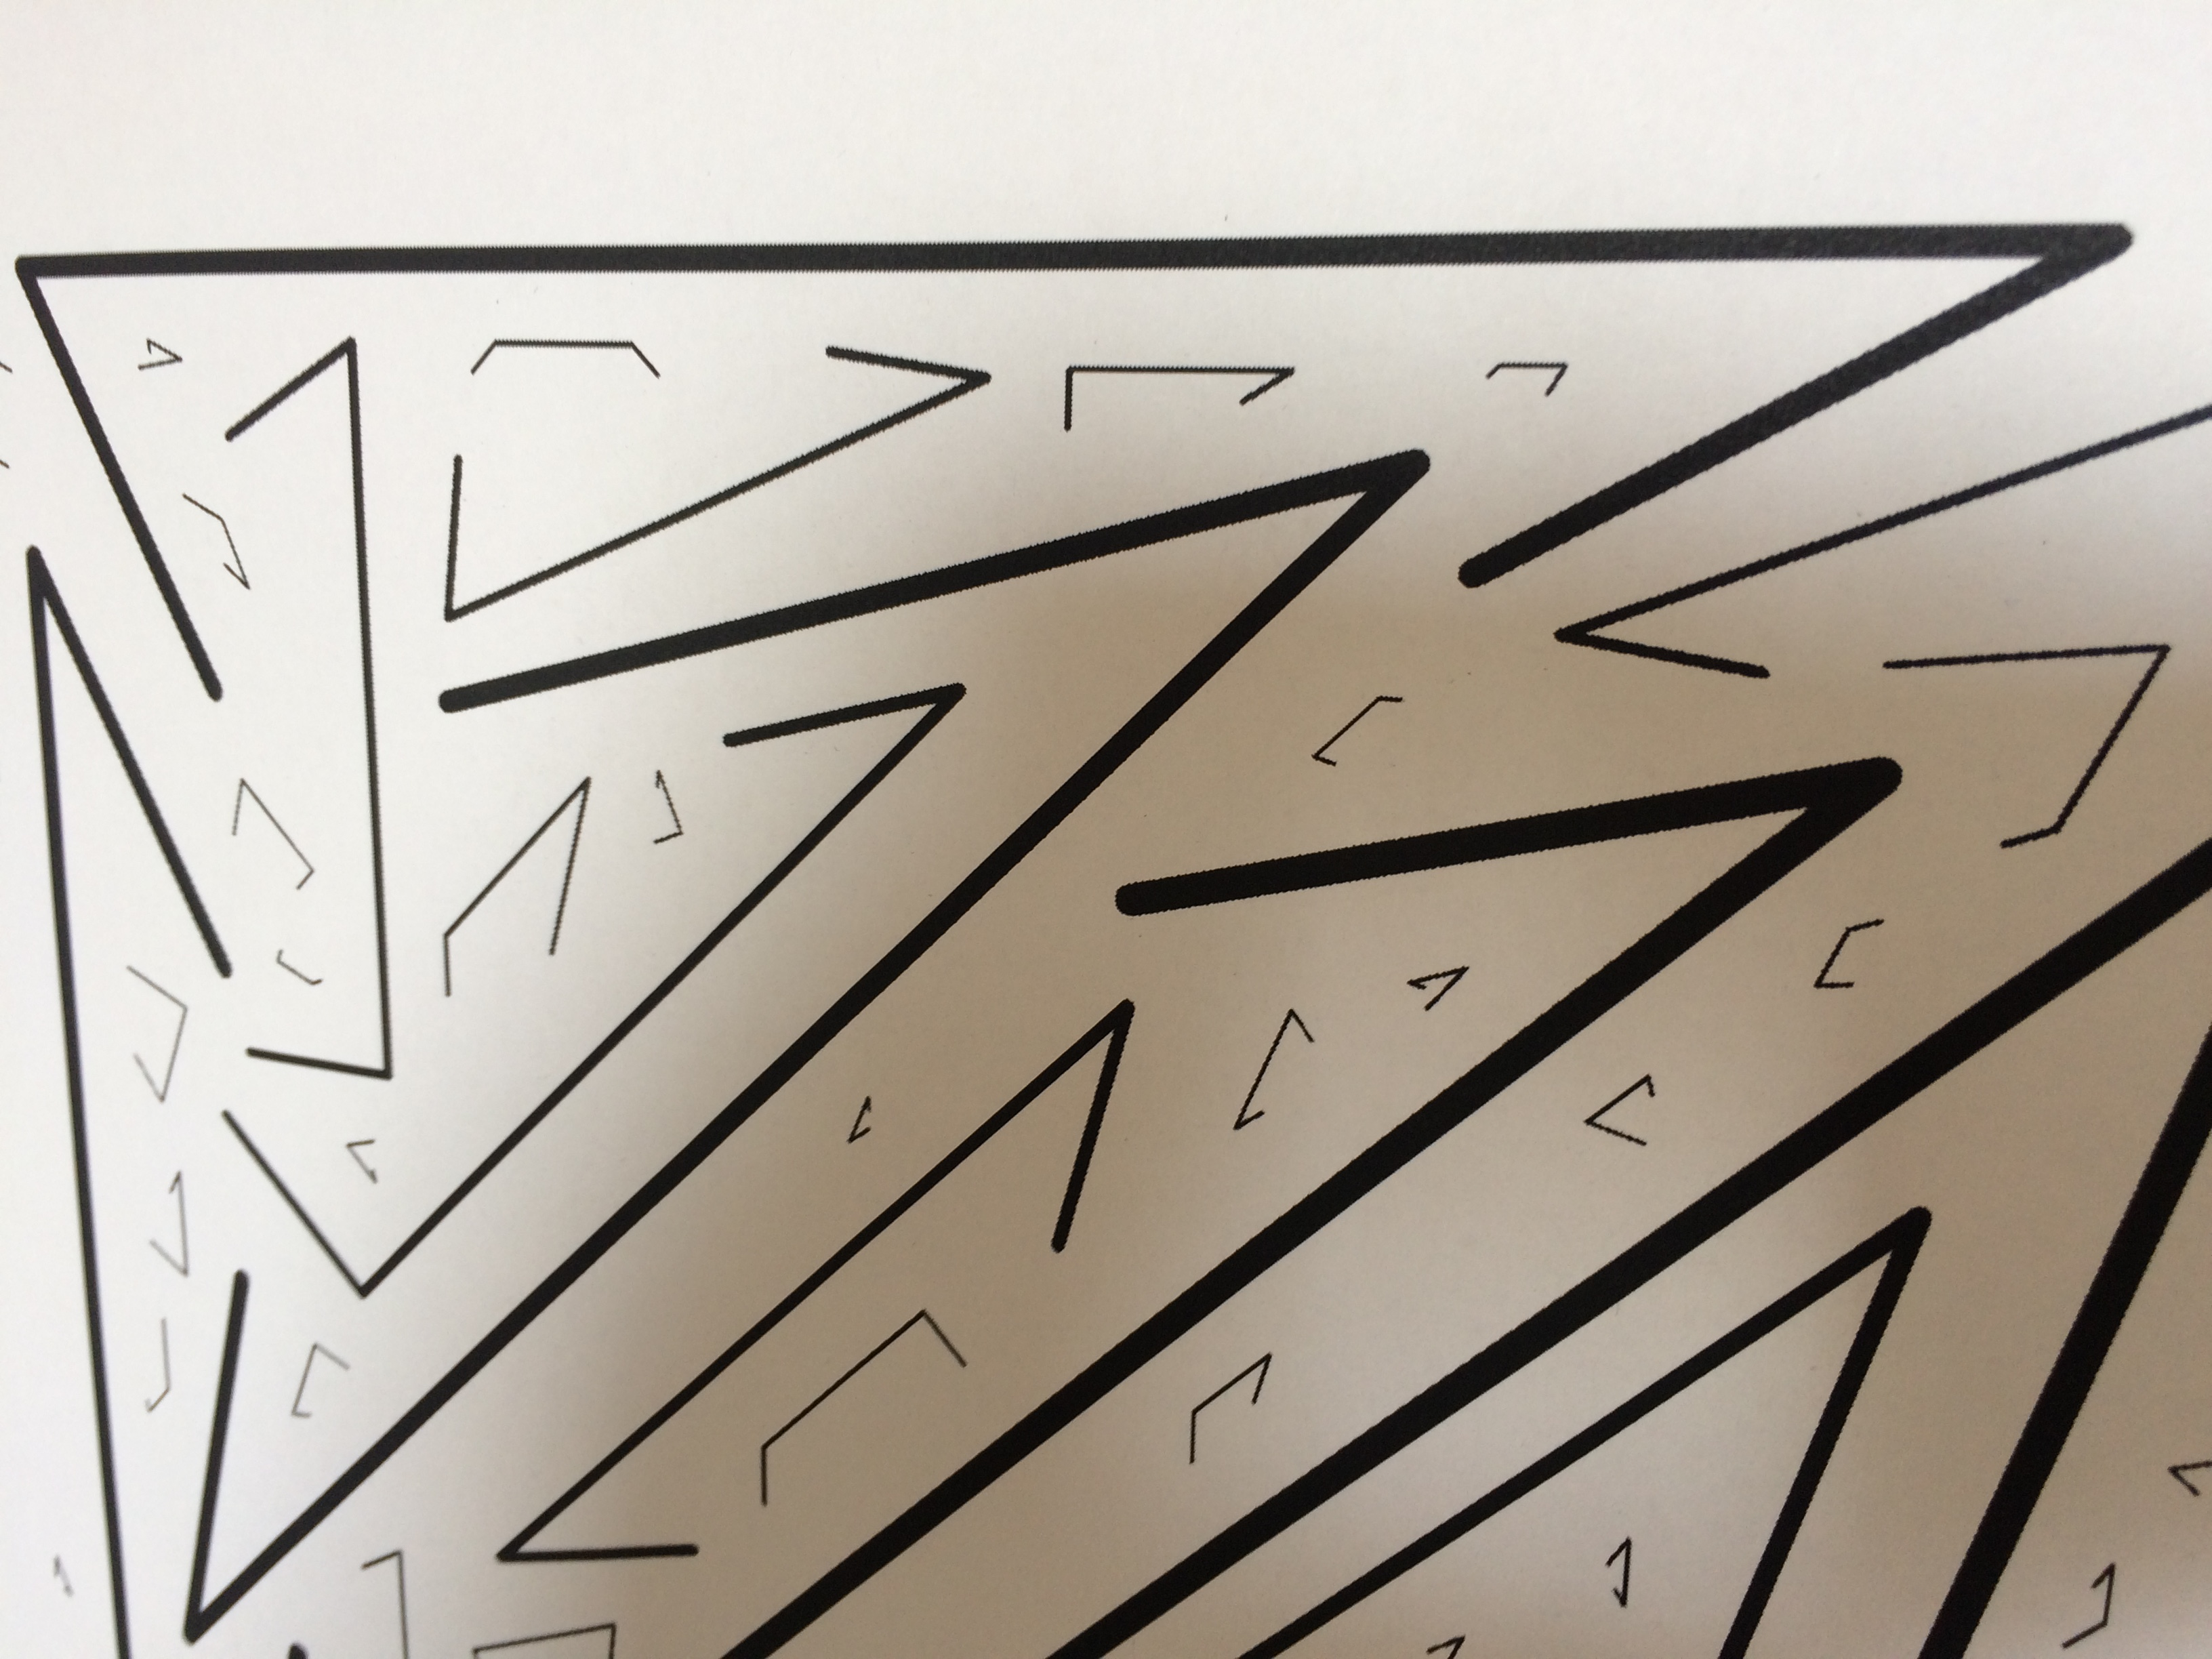
\includegraphics[width=0.75\textwidth]{figures/t35_01.JPG}
	\caption{Partially visible marker (taken with commercial smartphone)}
	\label{fig:partialMarkerShot}
\end{figure}


%-----------------------------------------------------------------------------------------------
\section{Theoretical Overview}
%-----------------------------------------------------------------------------------------------

%-----------------------------------------------------------------------------------------------
\subsection{Hough transformation}
%-----------------------------------------------------------------------------------------------

One of the most commonly used methods for line detection on images is the Hough transform.
Over it's long history many publications have been made about it's applications, performance and improvements.

Originally it was developed by Paul Hough in 1959 and later patented in 1962\cite{houghPatent}.
It was intended to be used for machine analysis of bubble chamber photographs.
In it's modern form (with the $\theta-\rho$ parametrisation) was introduced in 1972 by Duda and Hart\cite{houghThetaRho}.
The transformation became popular in the image processing community after Ballard's article\cite{BALLARD1981111} about generalising the algorithm for detection of arbitrary shapes.
There were many optimised and improved variants of the transformation, however the basic concept remained the same.
In 1990 a publication\cite{XU1990331} introduced the Randomized Hough Transform, which was a fundamentally new approach to the algorithm with notable merits.
As opposed to the one-to-many mapping of the simple Hough transform, the randomised version uses a convergent many-to-one mapping when creating the parameter space.

After this short historical overview the theory and the application of the transformation will be discussed.

%-----------------------------------------------------------------------------------------------
\subsubsection{Standard Hough Transform}
%-----------------------------------------------------------------------------------------------

The transformation is used to find instances of a model on digital images.
The models are usually simple geometric shapes like lines, circles or ellipses.
The curves are described by their parameters, e.g. slope and intercept for a line, centre point and radius for a circle etc..
Every non-zero pixel\footnote{The transformation works on binary images} votes for the features it could be part of.
The number of votes is stored for every possible parameter combination.
Then a threshold is applied to the stored votes, and the remaining parameters are accepted as model instances.
	
At first Hough described the algorithm to lines, but later the method would be generalised to any analytic\footnote{The Generalised Hough Transform even extends to arbitrary shapes} curve or shape.
This theoretical overview is based on the example of line detection.
The process is the same for every analytic curve, the only difference is the parameter space's dimension.
The original patent\cite{houghPatent} used the slope-intercept representation of lines.
\begin{equation}
y = m*x + b
\end{equation}
In this case, the \emph{parameter space} is 2 dimensional and it's axes are $m$ and $b$.
Every point in the parameter space represent an image space line.
With this representation every non-zero pixel in the image space transforms into a line in the parameter space.
For a given $(x_0,y_0)$ pair \eqref{houghLineMB} gives the line in the parameter space. 
\begin{equation}
\label{eq:houghLineMB}
b = -x_0*m + y_0
\end{equation}
Collinear points in the image show up in the parameter space as intersecting lines.
The more lines intersect in a given $(m_0,b_0)$, the more likely it is the image contains the $y = m_0*x + b_0$ line.
The problem with this parametrisation is that the parameter space is unbounded along both axes.
Both intersect and slope can have values in the range of $(-\infty, \infty)$.
Duda and Hart\cite{houghThetaRho} proposed an alternative parametrisation, which turned out to be better for application.
They used the \emph{normal parametrisation} of a line, shown in \eqref{normalParams}.
\begin{equation}
	\label{eq:normalParams}
	\rho = x*cos(\theta) + y*sin(\theta)
\end{equation}
In \eqref{normalParams} $\rho$ means the distance of the line from the image plane's origin.
$\theta$ is angle of the normal vector of the line.
\begin{figure}[ht]
	\centering
	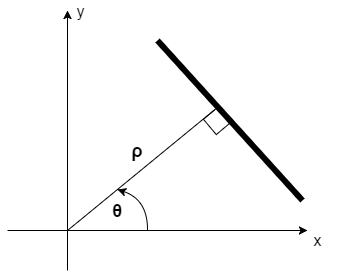
\includegraphics[width=0.5\textwidth]{figures/line_params.png}
	\caption{Normal line parameters}
	\label{fig:normalLineParams}
\end{figure}
If the \emph{normal parametrisation} is used the parameter space becomes finite in both dimensions.
$\theta$ is in the range of $(0,2\pi)$, $\rho$ is bounded by the image size.
In this case the image points define sinusoid curves in the parameter plane, and the line detection is done by searching for their intersections.
\begin{figure}[ht]
	\centering
	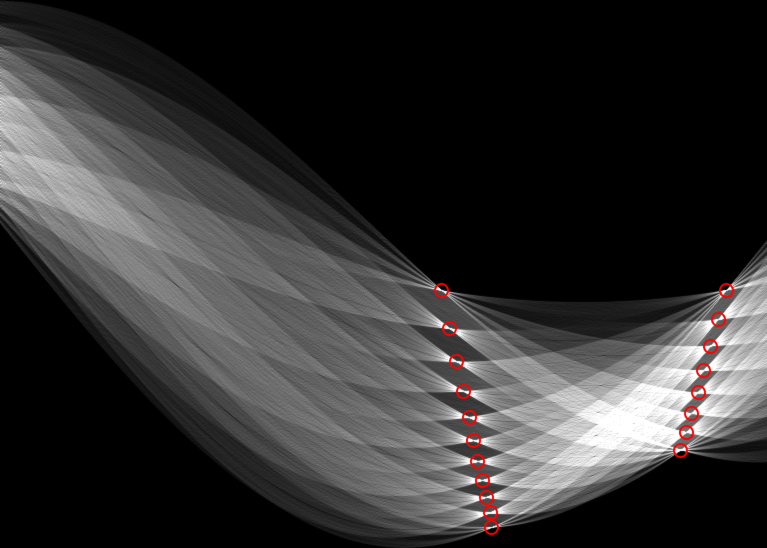
\includegraphics[width=0.6\textwidth]{figures/Perspective_chessboard_hough_transform.png}
	\caption{Hough-transform of a chessboard pattern}
	\label{fig:houghChessBoard}
\end{figure}

As mentioned before, the line detection is based on a voting scheme.
The parameter space (in this case a 2 dimensional plane) is divided into \emph{bins}.
$\rho$ and $\theta$ are quantised in the desired resolution.
The discrete $(\rho,\theta)$ pairs define the bins.
Every bin has accumulator.
When a given $(\rho_i,\theta_i)$ pair gets a vote it's corresponding accumulator is incremented by 1.
The \textbf{SHT} (Standard Hough Transform) uses one-to-many divergent mapping.
This means that every non-zero pixel votes for every possible parameter pair it could belong to.
The above mentioned sinusoid is calculated with the desired resolution for the pixel, and the corresponding accumulators are updated.

When the accumulation phase is completed for the whole image, the local maxima of the accumulators are found.
Usually a threshold is applied in order to reduce noise and eliminate too short line segments.
The radius of the non-maxima suppression also has impact on the results of the line fitting, it must be chosen carefully.
After this step the parameters for the most likely line candidates are available.

As the \textbf{SHT} does not provide the endpoints of the line, they must be found by examining the original binary image.
This can be done by simple checking every pixel along the line with the given parameters and deciding whether or not it is part of the feature.
If it is desired, lines with gaps can also be accepted with this method.
For more accurate fitting, a Least Squares approximation can also be applied to the pixels belonging to the line.

%-----------------------------------------------------------------------------------------------
\subsubsection{Randomized Hough Transform}
%-----------------------------------------------------------------------------------------------

%-----------------------------------------------------------------------------------------------
\subsection{Corner Detection}
%-----------------------------------------------------------------------------------------------


%-----------------------------------------------------------------------------------------------
\subsection{Line Segment Detector}
%-----------------------------------------------------------------------------------------------

%-----------------------------------------------------------------------------------------------
\section{Application for Quad Detection}
%-----------------------------------------------------------------------------------------------


%-----------------------------------------------------------------------------------------------
\subsection{Conditioning}
%-----------------------------------------------------------------------------------------------

Before running the line detection algorithms some conditioning steps are done in order to improve their effectiveness.
These processes are not uniform - every fitting method needs it's own.

The Hough transformation traditionally works best on thin lines.
The easiest way is to generate an edge image with high-pass filtering.
The OpenCV framework offers a wide variety of features for this task.
The best result are obtained by using the Canny edge detector.

The skeletoning detector does not need a conditioning step, as it performs the band thinning on it's own.

The methods based on image gradients and corner detection both require some level of smoothing on the picture.
In case of the corner detection the smoothing is useful for removing the false positive matches caused by the jagged edges, or in case os JPEG images the artefacts caused by the compression.
The gradient detector simply gives a more spread-out and easier to analyse result on a smoothly changing gradient than it would on strict edge.
The smoothing is also implemented using the OpenCV framework, which provides easy access to Gaussian filtering.
The OpenCV implementation is based on convolution with a configurable Gaussian kernel.
The kernel size and the deviation in $x$ and $y$ direction can be set.
The Gaussian kernel and the convolution itself is handled in the framework.


